\documentclass[11pt]{report}

\usepackage[T1]{fontenc}
\usepackage[utf8]{inputenc}
\usepackage{graphicx}
\usepackage{formula}
\begin{document}
{\huge{\textbf La operación de los circuitos de activacion con tiristores en convertidores CA-CD y CA-CA}\\\\}
{\Large Ernesto Alonso Partida Lopez}\\\\
{\Large Universidad Politecnica De La Zona Metropolitana De Guadalajara}\\\\
{\Large Mecatronica, 3 A}\\
\date 24 de septiembre 2019\\

\includegraphics[scale=1]{upzmg.jpg} 
\newpage
{\Huge Rectificador trifasico no controlado de media onda}\\\\

{\Large Hasta los años 70´s la mayor parte de la electtronica de potencia estaba basada en el uso de tiristores, para ser mas especificos, SCRs los cuales eran usados ocmo interruptores controlados.}
\begin{figure}[hbtp]
\caption{Tiristor SCR}
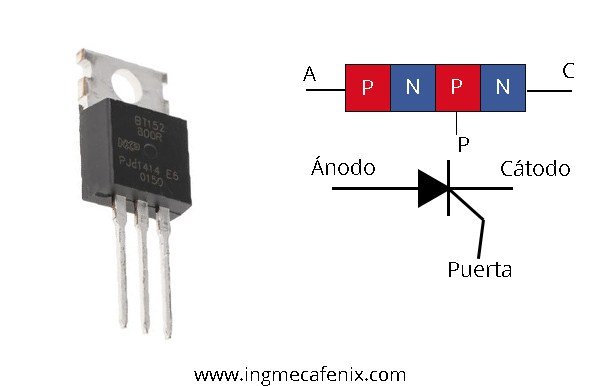
\includegraphics[scale=0.5]{../../../Downloads/descragas/Scr.jpg}
\end{figure}
 {\Large En la imagen 1 se muestra un tiristor los cuales pueden ser NPN o bien PNP esto dependiendo, dichos tiristores SCR, cuando estan incorporados a un circuito tienen la capacidad de rectificar un lado de la onda seniodal, e incluso tiene la habilidad de cortar la onda hasta el grado que se requiera para optener distintos resultados}
 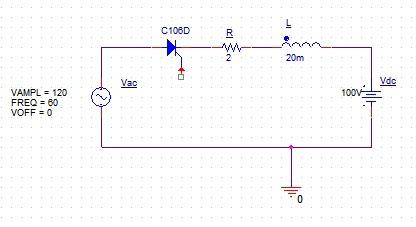
\includegraphics[scale=1]{../../../Downloads/descragas/Circuito753.jpg} 
 {\Large La imagen anterior nos muestra un circuito rectidficador de media onda en el cual se utilizan tiristores, para lo cual su onda sera similar a:}\\
 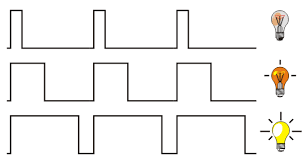
\includegraphics[scale=1]{../../../Downloads/descragas/images.png} 
 \newpage
 {\huge Rectificador trifasico no controlado de media onda}\\\\
 {\Large Existen dos diferentes tipo de rectificadores trifacicios no controlados los cuales puedes ser catodo comun o anodo comun, los cuales dependiendo de la posicion del tiristor este tiene su rectificaion ya sea en la parte de la onda positiva o en la parte negativa.}\\\\
{\huge Montaje en cátodo común}\\ 

	{\Large V{R}=V{G}* sen(2*3.14*F{red}*t) }\\\\
	{\Large V0med=({P}/{3.141})V* Sen({3.141}/{P})}\\\\
{\large Donde "P" es igual a las fases.}\\\\
{\huge Montaje en ánodo común}\\ 

	{\Large V{R}=V{G}* sen(2*3.14*F{red}*t) }\\\\
	{\Large V0med=-({P}/{3.141})V* Sen({3.141}/{P})}\\\\
	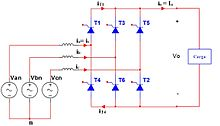
\includegraphics[scale=2]{../../../Downloads/descragas/220px-Rect_Trifasico_contr.jpg} \\
	\newpage
{\huge Rectificador trifasico no controlado de onda completa}\\\\
{\Large Existen dos diferentes tipos de circuito que nos permiten realizar una rectificacion de onda completa, los cuales son anodo comun y catado comun}\\

{\Large Vo=Vpo-VNo}\\\\
{\Large Vomed= 2(3/pi)Vg* sen(pi/3)\\\\
\begin{figure}[hbtp]
\centering
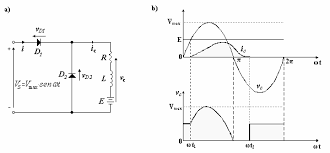
\includegraphics[scale=1]{../../../Downloads/descragas/images (1).png}
\caption{Onda completa}
\end{figure}
{\huge Rectificacion trifasico controlado}\\\\
{\Large Existen dos tipos de circuitos controlados los cuales puden ser de onda completa la cual consiste en rectificar ambos lados de la onda senoidal y por otro lado esta la de emdia onda la que puede ser rectificacion positiva o negativa esto dependiendo de la posicion de los tisristores}\\
\begin{figure}[hbtp]
\caption{Rectificacion controlada de media onda}
\centering
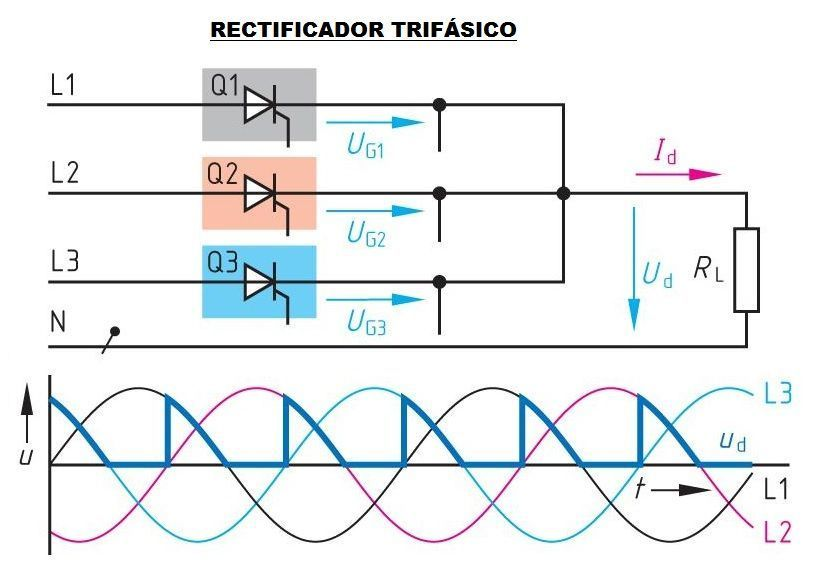
\includegraphics[scale=0.5]{../../../Downloads/descragas/a660ffbf974035d320255eb9fe1cafd4.jpg}
\end{figure}
\newpage
{\Huge BIbliografia}\\\\
@Book{Convertidores CA-CC y CA-CA con tiristores,
ALTauthor = {Pablo Termuro},
ALTeditor = {Convertidores CA-CC y CA-CA con tiristores},
title = {Convertidores CA-CC y CA-CA con tiristores},
publisher = {Ultima edicicon},
year = {2019},
OPTvolume = {1ro},
OPTedition = {monografias},
OPTmonth = {enero}
}




 
 
\end{document}